\chapter{Domain Model}
\label{chap:domainmodel}
\section{Domain Model}
\begin{figure}[H]
	\centering
    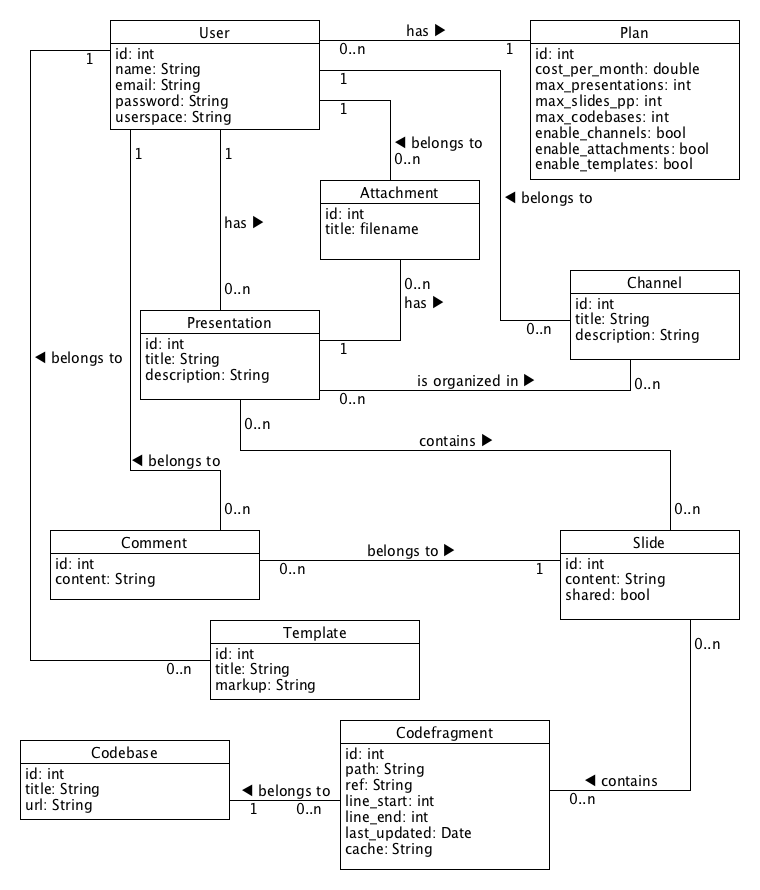
\includegraphics[width=1\textwidth]{images/domain-model.png}
    \caption{Domain Model}
\end{figure}

\section{Erläuterung zum Domain Model}


\subsection{User}
Ein User ist ein Benutzer des Systems. Er besitzt die gängigen Attribute für die Authentifizierung und Kommunikation. Ausserdem besitzt er ein Attribut \emph{userspace}, welches aussagt, wo seine \textbf{Attachments} abgelegt werden. Ein User kann weiter mehrere \textbf{Presentations} haben. Ausserdem kann ein User auch \textbf{Templates} haben. Zudem kann ein User auch \textbf{Channels} besitzen, um seine Präsentationen zu ordnen. Ein User hat auch immer einen \textbf{Plan}, welcher die Rechte vorgibt, die der User hat. Schliesslich werden alle \textbf{Comments} zu \textbf{Slides} einem User eindeutig zugeordnet.

\subsection{Plan}
Der Plan beschreibt die Rechte eines Users, also beispielsweise wie viele Präsentationen er anlegen kann oder wie viele Slides eine Präsentation haben kann.

\subsection{Presentation}
Eine Präsentation besitzt einen Titel und eine Beschreibung und gehört immer einem User. Eine Präsentation besetzt aus 0 bis n \textbf{Slides}. Eine Präsentation kann weiter zu einem oder mehreren Channels gehören. Um eine Präsentation zu erweitern, können ihr \textbf{Attachments} zugeordnet werden.

\subsection{Attachment}
Zu einem Attachment gehört der Filename. Jedes Attachment ist einem User zugeordnet.


\subsection{Channel}
Ein Channel dient zur Organisation von Präsentationen (beispielsweise pro Kurs, Modul, Thema, etc). Ein Channel kann mehrere Präsentationen enthalten. In der Zwischen-Entität (zwischen Channel und Präsentation) ist ausserdem definiert, in welcher Reihenfolge die Präsentationen im Channel erscheinen (als Linked-List implementiert).

\subsection{Slide}
Die Slides sind die Bestandteile der Präsentation. Eine Slide kann aber auch erstellt werden, ohne direkt einer Präsentation zugeordnet zu sein. Eine Slide hat einen Content (der Inhalt der Slide) und ein Flag, ob die Slide \emph{shared} ist, sprich zu mehreren Präsentationen gehört (für Titelfolien oder ähnliches). Eine Slide kann zudem auch \textbf{Codefragments} enthalten. Zudem ist jeder Kommentar (\textbf{Comment}) immer einer Slide zugeordnet.

\subsection{Comment}
Ein Comment wird von einem User zu einer Slide erfasst und besitzt einen Inhalt (\emph{content}).


\subsection{Codebase}
Die Codebases dienen zur Organisation von externen Code-Resourcen. In dieser Entität ist die \emph{url} hinterlegt, wo der Code geholt werden kann. Sie zeigt beispielsweise auf ein Git-Repository eines Users. Die Codebase hat dann für jedes Codestück (\textbf{Codefragment}) eine Beziehung in der Datenbank gespeichert. So kann, falls ein Repository gezügelt wird, nur die Codebase angepasst werden.

\subsection{Codefragment}
Die Entität Codefragment beschreibt einen Code-Ausschnitt. Das Fragment besitzt einen \emph{path}, welcher zur Datei im Repository zeigt. Mit dem \emph{ref} Field kann der Branch oder das Tag oder aber der Commit angegeben werden. Mit \emph{line_start} und \emph{line_end} wird beschrieben, welcher Ausschnitt aus der Datei geholt werden soll. Die Felder \emph{last_updated} und \emph{cache} dienen zur Zwischenspeicherung, damit der Code lokal (im System) gespeichert wird und nicht jedes mal neu geholt werden muss.


\section{Entity-Relationship Model}
\begin{figure}[H]
    \small \includesvg[width = 1\textwidth,pdf,path=images/]{erm}
    \caption{Entity-Relationship Model für die Datenmodellierung}
\end{figure}